% !TEX root = mythesis.tex

%==============================================================================
\chapter{Towards the Quark Mass Dependence of $T_{cc}(3875)$}
\label{sec:tcc}
% \newcommand{\todo}[1]{\textbf{\color{red}TODO: #1}}

%==============================================================================
In this section we briefly describe the remaining tasks and the end goals of this project which will comprise a Doctoral thesis. We begin with a brief forary into multi-hadron interpolators with charm quarks and exotic hadrons. We endeavor to perform a rigourous analysis of the dependence of energy spectra and scattering phase shifts on the degree of distillation smearing. Our testing ground will be the single and double pion system for a collection of covariant derivatives and total momenta. This analysis for hadrons containing charm quarks will then follow suit. In this vein, the remaining tasks are 
\begin{itemize}
    \item computation of spectrum for a range of center-of-mass momenta in various irreps of $O_h$
    \item Finite volume analysis of the discrete spectrum on several volumes and momentum frames
    \item Extract isospin-1 P-wave scattering phase shift 
    \item Determine the systematic uncertainty coming from $m_\pi$ 
    \item $T_{cc}^+$ dependence on $m_\pi$ as the latter approaches the physical point
\end{itemize}


\section{Exotic Hadrons in a (very small) nutshell}
Since the turn of the century, collider experiments have identified resonances that do not fit into the traditional quark model; The two competing hypotheses are that these states are either bound states of di-quarks and anti-di-quarks (tetraquarks) or di-meson states. 
For comprehensive reviews the topic, see \cite{Chen}\cite{Guo:2017jvc} \cite{Brambilla:2019esw}We aim to confirm that the doubly charmed tetrqaurk state of interest is a member of the class of hadrons shown in g

\begin{figure}[h]
    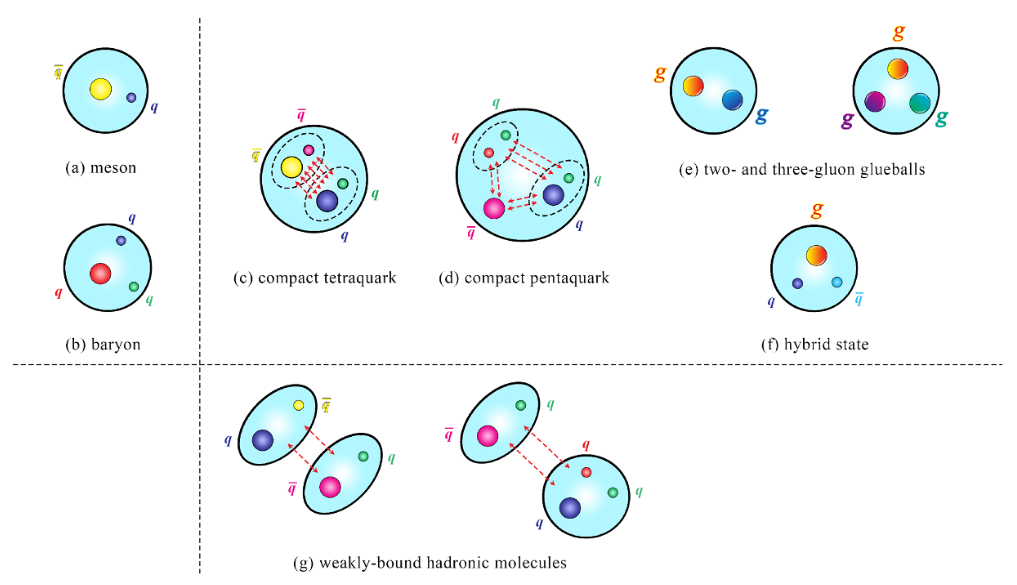
\includegraphics[width=1.0\textwidth, inner]{hadron_states.png}
    \caption{different structures of hadrons with emphasis on the di-meson state in (g) and the tetraquark state in (c)}
    \label{fig:figure6}
    \end{figure}
The particular color structure of a tetraquark that we will investigate is the hadronic molecule type 
\begin{equation}
    3_q \otimes 3_q \otimes \bar{3}_{\bar{q}} \otimes \bar{3}_{\bar{q}} \rightarrow 1_{[\bar{q}q]_1[\bar{q}q]_1} \rightarrow \delta_{ab} \delta_{cd} \times \bar{q}^aq^b\bar{q}^cq^d 
\end{equation}
Where $a..d = 1..3$ and $n=1...8$ are the color indices. 

The flavor $SU(3)$ representations of the tetraquark states are 
\begin{align}
& 3_q \otimes 3_q \otimes \bar{3}_{\bar{q}} \otimes \bar{3}_{\bar{q}} \nonumber \\
& = (1 \oplus 8)_{[qq]_{\bar{3}}[\bar{q}\bar{q}]_3} \oplus (8 \oplus 10)_{[qq]_6[\bar{q}\bar{q}]_3} \nonumber \\
& \oplus (8 \oplus \bar{10})_{[qq]_{\bar{3}}[\bar{q}\bar{q}]\bar{6}} \oplus (1 \oplus 8 \oplus 27)_{[qq]_6[\bar{q}\bar{q}]_{\bar{6}}}
\end{align}

\section{Multi-Hadron Interpolating Operators with charm quarks}
There is a vast amount of literature on computing the Charmonium spectrum with LQCD. See \todo{insert charm cites}

First, we must calculate the energy levels of the $T_{cc}$, then extract the scattering amplitude and the poles therein. 

\begin{enumerate}
    \item compute spectrum for a range of:
    \subitem center-of-mass momenta 
    \subitem in various irreducible representations of the relevant symmetry group, which in this case, is the octahedral group $O_h^D$ 
    \item Perform a finite volume analysis of the discrete spectrum on several mvolumes and momentum frames
        \subitem \textbf{Note: Hadrons containing heavy quarks are prone to discretization errors thus a controlled continuum limit at finite lattice spacing is required} 
    \item determine values of the isospin-1 P-wave scattering phase shift 
\end{enumerate}
    